
% Default to the notebook output style

    


% Inherit from the specified cell style.




    
\documentclass[11pt]{article}

    
    
    \usepackage[T1]{fontenc}
    % Nicer default font (+ math font) than Computer Modern for most use cases
    \usepackage{mathpazo}

    % Basic figure setup, for now with no caption control since it's done
    % automatically by Pandoc (which extracts ![](path) syntax from Markdown).
    \usepackage{graphicx}
    % We will generate all images so they have a width \maxwidth. This means
    % that they will get their normal width if they fit onto the page, but
    % are scaled down if they would overflow the margins.
    \makeatletter
    \def\maxwidth{\ifdim\Gin@nat@width>\linewidth\linewidth
    \else\Gin@nat@width\fi}
    \makeatother
    \let\Oldincludegraphics\includegraphics
    % Set max figure width to be 80% of text width, for now hardcoded.
    \renewcommand{\includegraphics}[1]{\Oldincludegraphics[width=.8\maxwidth]{#1}}
    % Ensure that by default, figures have no caption (until we provide a
    % proper Figure object with a Caption API and a way to capture that
    % in the conversion process - todo).
    \usepackage{caption}
    \DeclareCaptionLabelFormat{nolabel}{}
    \captionsetup{labelformat=nolabel}

    \usepackage{adjustbox} % Used to constrain images to a maximum size 
    \usepackage{xcolor} % Allow colors to be defined
    \usepackage{enumerate} % Needed for markdown enumerations to work
    \usepackage{geometry} % Used to adjust the document margins
    \usepackage{amsmath} % Equations
    \usepackage{amssymb} % Equations
    \usepackage{textcomp} % defines textquotesingle
    % Hack from http://tex.stackexchange.com/a/47451/13684:
    \AtBeginDocument{%
        \def\PYZsq{\textquotesingle}% Upright quotes in Pygmentized code
    }
    \usepackage{upquote} % Upright quotes for verbatim code
    \usepackage{eurosym} % defines \euro
    \usepackage[mathletters]{ucs} % Extended unicode (utf-8) support
    \usepackage[utf8x]{inputenc} % Allow utf-8 characters in the tex document
    \usepackage{fancyvrb} % verbatim replacement that allows latex
    \usepackage{grffile} % extends the file name processing of package graphics 
                         % to support a larger range 
    % The hyperref package gives us a pdf with properly built
    % internal navigation ('pdf bookmarks' for the table of contents,
    % internal cross-reference links, web links for URLs, etc.)
    \usepackage{hyperref}
    \usepackage{longtable} % longtable support required by pandoc >1.10
    \usepackage{booktabs}  % table support for pandoc > 1.12.2
    \usepackage[inline]{enumitem} % IRkernel/repr support (it uses the enumerate* environment)
    \usepackage[normalem]{ulem} % ulem is needed to support strikethroughs (\sout)
                                % normalem makes italics be italics, not underlines
    

    
    
    % Colors for the hyperref package
    \definecolor{urlcolor}{rgb}{0,.145,.698}
    \definecolor{linkcolor}{rgb}{.71,0.21,0.01}
    \definecolor{citecolor}{rgb}{.12,.54,.11}

    % ANSI colors
    \definecolor{ansi-black}{HTML}{3E424D}
    \definecolor{ansi-black-intense}{HTML}{282C36}
    \definecolor{ansi-red}{HTML}{E75C58}
    \definecolor{ansi-red-intense}{HTML}{B22B31}
    \definecolor{ansi-green}{HTML}{00A250}
    \definecolor{ansi-green-intense}{HTML}{007427}
    \definecolor{ansi-yellow}{HTML}{DDB62B}
    \definecolor{ansi-yellow-intense}{HTML}{B27D12}
    \definecolor{ansi-blue}{HTML}{208FFB}
    \definecolor{ansi-blue-intense}{HTML}{0065CA}
    \definecolor{ansi-magenta}{HTML}{D160C4}
    \definecolor{ansi-magenta-intense}{HTML}{A03196}
    \definecolor{ansi-cyan}{HTML}{60C6C8}
    \definecolor{ansi-cyan-intense}{HTML}{258F8F}
    \definecolor{ansi-white}{HTML}{C5C1B4}
    \definecolor{ansi-white-intense}{HTML}{A1A6B2}

    % commands and environments needed by pandoc snippets
    % extracted from the output of `pandoc -s`
    \providecommand{\tightlist}{%
      \setlength{\itemsep}{0pt}\setlength{\parskip}{0pt}}
    \DefineVerbatimEnvironment{Highlighting}{Verbatim}{commandchars=\\\{\}}
    % Add ',fontsize=\small' for more characters per line
    \newenvironment{Shaded}{}{}
    \newcommand{\KeywordTok}[1]{\textcolor[rgb]{0.00,0.44,0.13}{\textbf{{#1}}}}
    \newcommand{\DataTypeTok}[1]{\textcolor[rgb]{0.56,0.13,0.00}{{#1}}}
    \newcommand{\DecValTok}[1]{\textcolor[rgb]{0.25,0.63,0.44}{{#1}}}
    \newcommand{\BaseNTok}[1]{\textcolor[rgb]{0.25,0.63,0.44}{{#1}}}
    \newcommand{\FloatTok}[1]{\textcolor[rgb]{0.25,0.63,0.44}{{#1}}}
    \newcommand{\CharTok}[1]{\textcolor[rgb]{0.25,0.44,0.63}{{#1}}}
    \newcommand{\StringTok}[1]{\textcolor[rgb]{0.25,0.44,0.63}{{#1}}}
    \newcommand{\CommentTok}[1]{\textcolor[rgb]{0.38,0.63,0.69}{\textit{{#1}}}}
    \newcommand{\OtherTok}[1]{\textcolor[rgb]{0.00,0.44,0.13}{{#1}}}
    \newcommand{\AlertTok}[1]{\textcolor[rgb]{1.00,0.00,0.00}{\textbf{{#1}}}}
    \newcommand{\FunctionTok}[1]{\textcolor[rgb]{0.02,0.16,0.49}{{#1}}}
    \newcommand{\RegionMarkerTok}[1]{{#1}}
    \newcommand{\ErrorTok}[1]{\textcolor[rgb]{1.00,0.00,0.00}{\textbf{{#1}}}}
    \newcommand{\NormalTok}[1]{{#1}}
    
    % Additional commands for more recent versions of Pandoc
    \newcommand{\ConstantTok}[1]{\textcolor[rgb]{0.53,0.00,0.00}{{#1}}}
    \newcommand{\SpecialCharTok}[1]{\textcolor[rgb]{0.25,0.44,0.63}{{#1}}}
    \newcommand{\VerbatimStringTok}[1]{\textcolor[rgb]{0.25,0.44,0.63}{{#1}}}
    \newcommand{\SpecialStringTok}[1]{\textcolor[rgb]{0.73,0.40,0.53}{{#1}}}
    \newcommand{\ImportTok}[1]{{#1}}
    \newcommand{\DocumentationTok}[1]{\textcolor[rgb]{0.73,0.13,0.13}{\textit{{#1}}}}
    \newcommand{\AnnotationTok}[1]{\textcolor[rgb]{0.38,0.63,0.69}{\textbf{\textit{{#1}}}}}
    \newcommand{\CommentVarTok}[1]{\textcolor[rgb]{0.38,0.63,0.69}{\textbf{\textit{{#1}}}}}
    \newcommand{\VariableTok}[1]{\textcolor[rgb]{0.10,0.09,0.49}{{#1}}}
    \newcommand{\ControlFlowTok}[1]{\textcolor[rgb]{0.00,0.44,0.13}{\textbf{{#1}}}}
    \newcommand{\OperatorTok}[1]{\textcolor[rgb]{0.40,0.40,0.40}{{#1}}}
    \newcommand{\BuiltInTok}[1]{{#1}}
    \newcommand{\ExtensionTok}[1]{{#1}}
    \newcommand{\PreprocessorTok}[1]{\textcolor[rgb]{0.74,0.48,0.00}{{#1}}}
    \newcommand{\AttributeTok}[1]{\textcolor[rgb]{0.49,0.56,0.16}{{#1}}}
    \newcommand{\InformationTok}[1]{\textcolor[rgb]{0.38,0.63,0.69}{\textbf{\textit{{#1}}}}}
    \newcommand{\WarningTok}[1]{\textcolor[rgb]{0.38,0.63,0.69}{\textbf{\textit{{#1}}}}}
    
    
    % Define a nice break command that doesn't care if a line doesn't already
    % exist.
    \def\br{\hspace*{\fill} \\* }
    % Math Jax compatability definitions
    \def\gt{>}
    \def\lt{<}
    % Document parameters
    \title{Draft Submission}
    
    
    

    % Pygments definitions
    
\makeatletter
\def\PY@reset{\let\PY@it=\relax \let\PY@bf=\relax%
    \let\PY@ul=\relax \let\PY@tc=\relax%
    \let\PY@bc=\relax \let\PY@ff=\relax}
\def\PY@tok#1{\csname PY@tok@#1\endcsname}
\def\PY@toks#1+{\ifx\relax#1\empty\else%
    \PY@tok{#1}\expandafter\PY@toks\fi}
\def\PY@do#1{\PY@bc{\PY@tc{\PY@ul{%
    \PY@it{\PY@bf{\PY@ff{#1}}}}}}}
\def\PY#1#2{\PY@reset\PY@toks#1+\relax+\PY@do{#2}}

\expandafter\def\csname PY@tok@w\endcsname{\def\PY@tc##1{\textcolor[rgb]{0.73,0.73,0.73}{##1}}}
\expandafter\def\csname PY@tok@c\endcsname{\let\PY@it=\textit\def\PY@tc##1{\textcolor[rgb]{0.25,0.50,0.50}{##1}}}
\expandafter\def\csname PY@tok@cp\endcsname{\def\PY@tc##1{\textcolor[rgb]{0.74,0.48,0.00}{##1}}}
\expandafter\def\csname PY@tok@k\endcsname{\let\PY@bf=\textbf\def\PY@tc##1{\textcolor[rgb]{0.00,0.50,0.00}{##1}}}
\expandafter\def\csname PY@tok@kp\endcsname{\def\PY@tc##1{\textcolor[rgb]{0.00,0.50,0.00}{##1}}}
\expandafter\def\csname PY@tok@kt\endcsname{\def\PY@tc##1{\textcolor[rgb]{0.69,0.00,0.25}{##1}}}
\expandafter\def\csname PY@tok@o\endcsname{\def\PY@tc##1{\textcolor[rgb]{0.40,0.40,0.40}{##1}}}
\expandafter\def\csname PY@tok@ow\endcsname{\let\PY@bf=\textbf\def\PY@tc##1{\textcolor[rgb]{0.67,0.13,1.00}{##1}}}
\expandafter\def\csname PY@tok@nb\endcsname{\def\PY@tc##1{\textcolor[rgb]{0.00,0.50,0.00}{##1}}}
\expandafter\def\csname PY@tok@nf\endcsname{\def\PY@tc##1{\textcolor[rgb]{0.00,0.00,1.00}{##1}}}
\expandafter\def\csname PY@tok@nc\endcsname{\let\PY@bf=\textbf\def\PY@tc##1{\textcolor[rgb]{0.00,0.00,1.00}{##1}}}
\expandafter\def\csname PY@tok@nn\endcsname{\let\PY@bf=\textbf\def\PY@tc##1{\textcolor[rgb]{0.00,0.00,1.00}{##1}}}
\expandafter\def\csname PY@tok@ne\endcsname{\let\PY@bf=\textbf\def\PY@tc##1{\textcolor[rgb]{0.82,0.25,0.23}{##1}}}
\expandafter\def\csname PY@tok@nv\endcsname{\def\PY@tc##1{\textcolor[rgb]{0.10,0.09,0.49}{##1}}}
\expandafter\def\csname PY@tok@no\endcsname{\def\PY@tc##1{\textcolor[rgb]{0.53,0.00,0.00}{##1}}}
\expandafter\def\csname PY@tok@nl\endcsname{\def\PY@tc##1{\textcolor[rgb]{0.63,0.63,0.00}{##1}}}
\expandafter\def\csname PY@tok@ni\endcsname{\let\PY@bf=\textbf\def\PY@tc##1{\textcolor[rgb]{0.60,0.60,0.60}{##1}}}
\expandafter\def\csname PY@tok@na\endcsname{\def\PY@tc##1{\textcolor[rgb]{0.49,0.56,0.16}{##1}}}
\expandafter\def\csname PY@tok@nt\endcsname{\let\PY@bf=\textbf\def\PY@tc##1{\textcolor[rgb]{0.00,0.50,0.00}{##1}}}
\expandafter\def\csname PY@tok@nd\endcsname{\def\PY@tc##1{\textcolor[rgb]{0.67,0.13,1.00}{##1}}}
\expandafter\def\csname PY@tok@s\endcsname{\def\PY@tc##1{\textcolor[rgb]{0.73,0.13,0.13}{##1}}}
\expandafter\def\csname PY@tok@sd\endcsname{\let\PY@it=\textit\def\PY@tc##1{\textcolor[rgb]{0.73,0.13,0.13}{##1}}}
\expandafter\def\csname PY@tok@si\endcsname{\let\PY@bf=\textbf\def\PY@tc##1{\textcolor[rgb]{0.73,0.40,0.53}{##1}}}
\expandafter\def\csname PY@tok@se\endcsname{\let\PY@bf=\textbf\def\PY@tc##1{\textcolor[rgb]{0.73,0.40,0.13}{##1}}}
\expandafter\def\csname PY@tok@sr\endcsname{\def\PY@tc##1{\textcolor[rgb]{0.73,0.40,0.53}{##1}}}
\expandafter\def\csname PY@tok@ss\endcsname{\def\PY@tc##1{\textcolor[rgb]{0.10,0.09,0.49}{##1}}}
\expandafter\def\csname PY@tok@sx\endcsname{\def\PY@tc##1{\textcolor[rgb]{0.00,0.50,0.00}{##1}}}
\expandafter\def\csname PY@tok@m\endcsname{\def\PY@tc##1{\textcolor[rgb]{0.40,0.40,0.40}{##1}}}
\expandafter\def\csname PY@tok@gh\endcsname{\let\PY@bf=\textbf\def\PY@tc##1{\textcolor[rgb]{0.00,0.00,0.50}{##1}}}
\expandafter\def\csname PY@tok@gu\endcsname{\let\PY@bf=\textbf\def\PY@tc##1{\textcolor[rgb]{0.50,0.00,0.50}{##1}}}
\expandafter\def\csname PY@tok@gd\endcsname{\def\PY@tc##1{\textcolor[rgb]{0.63,0.00,0.00}{##1}}}
\expandafter\def\csname PY@tok@gi\endcsname{\def\PY@tc##1{\textcolor[rgb]{0.00,0.63,0.00}{##1}}}
\expandafter\def\csname PY@tok@gr\endcsname{\def\PY@tc##1{\textcolor[rgb]{1.00,0.00,0.00}{##1}}}
\expandafter\def\csname PY@tok@ge\endcsname{\let\PY@it=\textit}
\expandafter\def\csname PY@tok@gs\endcsname{\let\PY@bf=\textbf}
\expandafter\def\csname PY@tok@gp\endcsname{\let\PY@bf=\textbf\def\PY@tc##1{\textcolor[rgb]{0.00,0.00,0.50}{##1}}}
\expandafter\def\csname PY@tok@go\endcsname{\def\PY@tc##1{\textcolor[rgb]{0.53,0.53,0.53}{##1}}}
\expandafter\def\csname PY@tok@gt\endcsname{\def\PY@tc##1{\textcolor[rgb]{0.00,0.27,0.87}{##1}}}
\expandafter\def\csname PY@tok@err\endcsname{\def\PY@bc##1{\setlength{\fboxsep}{0pt}\fcolorbox[rgb]{1.00,0.00,0.00}{1,1,1}{\strut ##1}}}
\expandafter\def\csname PY@tok@kc\endcsname{\let\PY@bf=\textbf\def\PY@tc##1{\textcolor[rgb]{0.00,0.50,0.00}{##1}}}
\expandafter\def\csname PY@tok@kd\endcsname{\let\PY@bf=\textbf\def\PY@tc##1{\textcolor[rgb]{0.00,0.50,0.00}{##1}}}
\expandafter\def\csname PY@tok@kn\endcsname{\let\PY@bf=\textbf\def\PY@tc##1{\textcolor[rgb]{0.00,0.50,0.00}{##1}}}
\expandafter\def\csname PY@tok@kr\endcsname{\let\PY@bf=\textbf\def\PY@tc##1{\textcolor[rgb]{0.00,0.50,0.00}{##1}}}
\expandafter\def\csname PY@tok@bp\endcsname{\def\PY@tc##1{\textcolor[rgb]{0.00,0.50,0.00}{##1}}}
\expandafter\def\csname PY@tok@fm\endcsname{\def\PY@tc##1{\textcolor[rgb]{0.00,0.00,1.00}{##1}}}
\expandafter\def\csname PY@tok@vc\endcsname{\def\PY@tc##1{\textcolor[rgb]{0.10,0.09,0.49}{##1}}}
\expandafter\def\csname PY@tok@vg\endcsname{\def\PY@tc##1{\textcolor[rgb]{0.10,0.09,0.49}{##1}}}
\expandafter\def\csname PY@tok@vi\endcsname{\def\PY@tc##1{\textcolor[rgb]{0.10,0.09,0.49}{##1}}}
\expandafter\def\csname PY@tok@vm\endcsname{\def\PY@tc##1{\textcolor[rgb]{0.10,0.09,0.49}{##1}}}
\expandafter\def\csname PY@tok@sa\endcsname{\def\PY@tc##1{\textcolor[rgb]{0.73,0.13,0.13}{##1}}}
\expandafter\def\csname PY@tok@sb\endcsname{\def\PY@tc##1{\textcolor[rgb]{0.73,0.13,0.13}{##1}}}
\expandafter\def\csname PY@tok@sc\endcsname{\def\PY@tc##1{\textcolor[rgb]{0.73,0.13,0.13}{##1}}}
\expandafter\def\csname PY@tok@dl\endcsname{\def\PY@tc##1{\textcolor[rgb]{0.73,0.13,0.13}{##1}}}
\expandafter\def\csname PY@tok@s2\endcsname{\def\PY@tc##1{\textcolor[rgb]{0.73,0.13,0.13}{##1}}}
\expandafter\def\csname PY@tok@sh\endcsname{\def\PY@tc##1{\textcolor[rgb]{0.73,0.13,0.13}{##1}}}
\expandafter\def\csname PY@tok@s1\endcsname{\def\PY@tc##1{\textcolor[rgb]{0.73,0.13,0.13}{##1}}}
\expandafter\def\csname PY@tok@mb\endcsname{\def\PY@tc##1{\textcolor[rgb]{0.40,0.40,0.40}{##1}}}
\expandafter\def\csname PY@tok@mf\endcsname{\def\PY@tc##1{\textcolor[rgb]{0.40,0.40,0.40}{##1}}}
\expandafter\def\csname PY@tok@mh\endcsname{\def\PY@tc##1{\textcolor[rgb]{0.40,0.40,0.40}{##1}}}
\expandafter\def\csname PY@tok@mi\endcsname{\def\PY@tc##1{\textcolor[rgb]{0.40,0.40,0.40}{##1}}}
\expandafter\def\csname PY@tok@il\endcsname{\def\PY@tc##1{\textcolor[rgb]{0.40,0.40,0.40}{##1}}}
\expandafter\def\csname PY@tok@mo\endcsname{\def\PY@tc##1{\textcolor[rgb]{0.40,0.40,0.40}{##1}}}
\expandafter\def\csname PY@tok@ch\endcsname{\let\PY@it=\textit\def\PY@tc##1{\textcolor[rgb]{0.25,0.50,0.50}{##1}}}
\expandafter\def\csname PY@tok@cm\endcsname{\let\PY@it=\textit\def\PY@tc##1{\textcolor[rgb]{0.25,0.50,0.50}{##1}}}
\expandafter\def\csname PY@tok@cpf\endcsname{\let\PY@it=\textit\def\PY@tc##1{\textcolor[rgb]{0.25,0.50,0.50}{##1}}}
\expandafter\def\csname PY@tok@c1\endcsname{\let\PY@it=\textit\def\PY@tc##1{\textcolor[rgb]{0.25,0.50,0.50}{##1}}}
\expandafter\def\csname PY@tok@cs\endcsname{\let\PY@it=\textit\def\PY@tc##1{\textcolor[rgb]{0.25,0.50,0.50}{##1}}}

\def\PYZbs{\char`\\}
\def\PYZus{\char`\_}
\def\PYZob{\char`\{}
\def\PYZcb{\char`\}}
\def\PYZca{\char`\^}
\def\PYZam{\char`\&}
\def\PYZlt{\char`\<}
\def\PYZgt{\char`\>}
\def\PYZsh{\char`\#}
\def\PYZpc{\char`\%}
\def\PYZdl{\char`\$}
\def\PYZhy{\char`\-}
\def\PYZsq{\char`\'}
\def\PYZdq{\char`\"}
\def\PYZti{\char`\~}
% for compatibility with earlier versions
\def\PYZat{@}
\def\PYZlb{[}
\def\PYZrb{]}
\makeatother


    % Exact colors from NB
    \definecolor{incolor}{rgb}{0.0, 0.0, 0.5}
    \definecolor{outcolor}{rgb}{0.545, 0.0, 0.0}



    
    % Prevent overflowing lines due to hard-to-break entities
    \sloppy 
    % Setup hyperref package
    \hypersetup{
      breaklinks=true,  % so long urls are correctly broken across lines
      colorlinks=true,
      urlcolor=urlcolor,
      linkcolor=linkcolor,
      citecolor=citecolor,
      }
    % Slightly bigger margins than the latex defaults
    
    \geometry{verbose,tmargin=1in,bmargin=1in,lmargin=1in,rmargin=1in}
    
    

    \begin{document}
    
    
    \maketitle
    
    

    ---
title: Association-Risk: An Alternative Use for Natural Language Processing on the Johannesburg Stock Exchange (JSE)

author:
- Marcus Gawronsky
- Christpher Kleweg
- Robert Brink
- Ryan Kruger

date: 19 September 2018

abstract : A recent topic of interest in the realm of financial research has been the use of Artificial Intelligence (AI) in financial prediction. This paper explores the use of various techniques in the realm of Natural Language Processing, a popular computational technique in deriving meaning from text data, to analyze the relationship between company association and portfolio diversification for companies on the Johannesburg Stock Exchange (JSE). Using a novel take on the Word2Vec word embedding technique, we show word-vector association between companies to track portfolio volatility over time. 

pagenumbering: true


papersize: a4

biblio-title: Bibliography   
bibliography: library.bib
csl: harvard-university-of-cape-town.csl

---
    \hypertarget{abstract}{%
\section{Abstract}\label{abstract}}

A recent topic of interest in the realm of financial research has been
the use of Artificial Intelligence (AI) in financial prediction. This
paper explores the use of various techniques in the realm of Natural
Language Processing, a popular computational technique in deriving
meaning from text data, to analyze the relationship between company
association and portfolio diversification for companies on the
Johannesburg Stock Exchange (JSE). Using a novel take on the Word2Vec
word embedding technique, we show word-vector association between
companies to track portfolio volatility over time.

\hypertarget{introduction}{%
\section{Introduction}\label{introduction}}

With the ever-increasing availability of qualitative financial
information in the form of news articles, blog posts, message boards and
financially based social networks investors are no longer able to
efficiently monitor and process massive amounts of unstructured data
{[}@Tirunillai2012{]}. @Engelberg2008 observes that whilst some
financial information is still quickly incorporated into markets due to
its ease of understanding, investors tend to under-react to new
information that may be more ambiguous or costly to process. As a
result, a central focus of Natural Language Processing in the financial
domain thus far has been sentiment analysis, providing hedge fund
managers with a tool in efficiently processing information and hence the
ability to profit on potential market inefficiencies.
{[}@Engelberg2008{]}. In practice however, using sentiment analysis to
predict stock prices has shown limited success as ambiguity and
implicitly expressed sentiment remain challenging for computer
algorithms to interpret. While NLP tools may not be exceptionally
accurate at predicting sentiment, they are extremely good at making
associations between words and their contexts in text data. Therefore,
this paper presents an alternative use case of NLP in predicting
association risk of companies within a portfolio on the Johannesburg
Stock Exchange (JSE).

A widely debated topic in the field of financial research concerns the
measurement of financial risk. The Capital Asset Pricing Model (CAPM)
remains at the core of modern financial theory some 50 years after its
initial development by providing investors with a framework in
determining how the expected return of an investment is affected but its
risk. Central to the CAPM model is the assumption of efficient markets,
whereby investors are able to fully diversify away non-systematic risk
leaving systematic risk, represented by Beta, as the sole risk
determinant in calculating returns {[}@Strugnell2015{]}. Given markets
are shown not to be efficient in practice, we can conclude that
non-systematic risk is in fact a determinant of market returns. This is
supported by existing literature identifying non-systematic anomalies
such as the size effect {[}@Banz1981{]} and value effect
{[}@Basu1983{]}, both of which are shown to have reliable predictive
power in explaining returns. Sources of non-systematic risk can be
difficult to quantify, but may relate to the extent to which a portfolio
is diversified. While investors may choose to diversify across a number
of metrics present in the literature such as size, value or leverage,
the degree of association between companies remains a critical metric
reliant on analyst insights. Association can come from companies sharing
similar industries, sentiment, status, position in analyst insight or
subsidiary relationship. One challenge is how to both extract and
quantify these measures in a way that is both unbiased, scalable and
computationally tractable. We propose a method, using dynamic
document-vectors learned from a corpus derived from a 30-day news cycles
in order to quantify the association between companies in a portfolio.

This paper suggests an alternative risk metric to Beta known as
``association risk'' which measures the amount of association between
companies within a portfolio and hence its associated level of
diversification. This is achieved through the use sentiment analysis to
form rich vector representations of companies. Portfolios are then
formed at random using the sum of the distances between the companies in
vector space. Portfolios of greater sum distances imply less association
between companies and hence greater portfolio diversification. This
paper shows that portfolios with greater level of diversification
exhibit lower levels of volatility and therefore lower levels of risk.

\[\text{Association}=(\sum_{i=1}^{p} \sum_{j=1}^{p} \text{similarity}_{i,j})^{-1}\]

\[\text{similarity}_{i,j} = \cos(\theta) = {\mathbf{C}_{i} \cdot \mathbf{C}_{j} \over \|\mathbf{C}_{i}\| \|\mathbf{C}_{j}\|} = \frac{ \sum\limits_{k=1}^{n}{C_{i,k}  C_{j,k}} }{ \sqrt{\sum\limits_{k=1}^{n}{C_{i,k}^2}}  \sqrt{\sum\limits_{k=1}^{n}{C_{j,k}^2}} }\]

Association is calculated as the inverse of the sum of the cosine
distances between all document vectors calculated from a given news
window at some point in time. In the equation above \(p\) represents the
size the a given portfolio, \(C\) represent a given document vector
representing a company and \(k\) represents the \(k\) 'th element of a
vector.

This paper is organised as follows. Section 2 reviews the literature on
Natural Language Processing. Section 3 details the data, exploratory
analysis and method. In the exploratory analysis, this paper compares
four different techniques in drawing association between companies on
the JSE, namely LDA, LSI, Word2Vec and Doc2Vec. Section 4 contains the
results of this study and is split into two main sections being Date
ANCOVA and Portfolio ANCOVA, presenting our findings in a detailed
discussion. Finally in Section 5, we summarise and conclude our
findings.

\hypertarget{literature-review}{%
\section{Literature Review}\label{literature-review}}

The realm of Natural Language Processing (NLP) has seen increased
application in recent years with the growth of new techniques, datasets
and computing capacity {[}@Sohangir2018, @OLeary2009, @Cortis2017{]}. In
English, different words and phrases can share or have different
meanings. A key challenge of NLP comes in how to group these words and
phrases in a way which is automated and efficient.

Bag-of-Words (BOW) is one of the earliest iterations of NLP and while it
has many drawbacks {[}@Harris1954{]}, it does produce document vectors
which capture the common meaning of documents sharing the same words.
One disadvantage in the non-parametric Bag-of-Words technique is that it
does not weight words based on their distinctiveness in the corpus of
documents. Articles like \emph{`a'} or \emph{`the'} occur throughout all
English text, but contribute little meaning to a given sentence. While
much work has been done analysing the information in a given piece of
text {[}@Shannon1951{]}, term-frequency re-weighting has been a common
staple with the Bag-of-Words approach to document vectorization
{[}@SparckJones1972, @Robertson2004{]}. While this technique can
increase the sparsity of a given document vector, it can improve the
performance of document similarity measures, valuable in topic analysis
and document clustering {[}@Huang2008{]}.

Unsupervised techniques for dimensionality reduction have been popular
extensions on the Bag-of-Words approach. Papers by @Dumais1988 and
@Deerwester1990, through a technique called Latent Semantic Indexing
(LSI), compare the use of Factor Analysis (FA), Principal Component
Analysis (PCA) and Multidimensional Scaling (MDS) on count vectors. A
generative approach by @Blei2003, referred to as Latent Dirichlet
Allocation (LDA), uses a three-level hierarchical Bayesian model to
extract document vectors from a given corpus. This technique can be
computationally challenging but has become a staple in many online
applications. While LSI and LDA have demonstrated significant
improvements to document vectorization or embedding, works by
@Shannon1951 and @Huang1993 seem to indicate that a word's meaning can
be derived from the contexts it and other words find themselves in
rather than just their frequency {[}@Baroni2014{]}. These contexts,
known as skip-grams, refer to a sequence of words surrounding a target
word.

In a paper by @Bengio2003, a feed-forward neural network is used with
one hidden layer to predict a word's skip-gram {[}@Alexandrescu2006{]}.
Using the output of this hidden layer, @Bengio2003 demonstrate the value
of this approach in extracting rich word-vectors which accurately
capture the semantic meaning of words in a continuous vector space.
While this technique remains tractable on small datasets and
dictionaries, a breakthrough came with @Mikolov2013a and @Mikolov2013b
who used negative sampling on words' skip-grams as a tool to
re-parameterize the model into something more computationally tractable
{[}@Goldberg2014{]}. This technique has been extended by @Quoc2014 in a
method commonly referred to as Doc2Vec, which aims to find documents
representations by using the same negative sample technique discussed by
@Mikolov2013b.

Word2vec, introduced by @Mikolov2013a, is seen to be a very popular
technique across Machine Learning Methodologies for its ability to
create state-of-the-art word embeddings. Word2vev is a neural network
method used to produce high-dimensional vector representations of each
word or document in a vector space. Locations of the words relevant to
each other in the vector space determine the semantic relationships
between the words and Word2Vec is able to capture sentiment based
similarity between words. Word2vec can be implemented using continuous
Bag-of-Words (CBOW) and skip-gram approaches. In the original study the
quality of vector representations was evaluated using an analogical
reasoning task {[}@Mikolov2013a{]}. This used five types of semantic
language questions and nine types of syntactic questions. The questions
were created firstly by manually pairing lists of similar words and
thereafter questions were created by connecting two pairs. For example,
a list of 68 american cities and the states they belong to was made. The
question was correctly answered if the closest word to the vector
computed is the same as the question. Questions were correctly answered
with an accuracy of around 60\% {[}@mikolov2013a{]}. In a follow-up
study using the same analogical reasoning task {[}@mikolov2013a{]},
@Mikolov2013b used the skip-gram model accompanied by various new
efficiency techniques such as negative sampling, hierarchical softmax
and the subsampling of frequent words which markedly improved results
with an accuracy of 72\%.

Whilst Word2Vec has shown success in these applications
{[}@mikolov2013a, @mikolov2013b{]}, its use in the prediction of both
sentiment and stock price has shown limited success {[}@Quoc2014,
@Cortis2017, @Sohangir2018{]}. While many explanations may exist for
these findings, one primary reason can be drawn from the technique
itself; while negative sampling methods do provide semantically
meaningful word embeddings in a high dimensional vector space, there
exists no surety that some function exists to map these word vectors to
some sentiment domain, given that these embeddings are trained on
context rather than sentiment. Additionally, parsing is an issue when
sentiments associated with words becomes too rich, forming knots.

With the growing complexity of quantitative techniques in price
prediction , there remains a growing need for portfolio validation using
non-market data. With the rise of `black box' style models such as
neural networks and random forests, this validation remains increasingly
important as these models exhibit potential problems such as
overfitting, reduced transparency and biased results based on poor
sample data {[}@Glowacki2017{]}.

The problem with association-based metrics has been the difficulty of
extracting association from large data sets of news and research reports
as many techniques that try to compute association do not scale to large
corpora. Word2Vec scales on text data thanks to its feed-forward neural
network re-parameterization and use of skip-grams, we propose a
technique which derives an association based portfolio risk metric using
unstructured data, using both news articles and analyst reports.

\hypertarget{data-exploratory-analysis-and-method}{%
\section{Data, Exploratory Analysis and
Method}\label{data-exploratory-analysis-and-method}}

\hypertarget{data}{%
\subsection{Data}\label{data}}

This paper uses news articles obtained from multiple online sources, as
shown in Table 1. These websites were scraped for articles containing a
predefined dictionary of company names from the Johannesburg Stock
Exchange (JSE). Articles were scraped as at 12 July 2018, using the
Scrapy html parsing library and stored in comma separated files. The
articles were then grouped by day, before being grouped into sets of
30-day news cycles, ensuring the proper alignment of calendar days
against trading days.

Total Index Return was used in this study as a robust measure of price
in order to account for the effect of dividend payments. Price data was
sourced using the Reuters Datastream Service from companies on the
Johannesburg Stock Exchange between 16 May 2003 and 17 May 2018. A total
of 82 of the 174 JSE stocks were used due of volume of articles for
companies and access to their descriptions.

\hypertarget{exploratory-analysis}{%
\subsection{Exploratory Analysis}\label{exploratory-analysis}}

A number of techniques remain popular within the literature of NLP.
These include LDA, LSI, Doc2Vec and Word2Vec amongst others. In the
following section we analyze these four techniques and aim to visualize
their data in order to asses their power in drawing association between
companies on the JSE.

Models are first trained on a fixed dataset of company descriptions.
Document vectors are then computed using these various models
representing each company. Two techniques were used in order to
visualize these 100-dimensional document vectors, namely t-distributed
Stochastic Neighbour Embedding (tSNE), a popular manifold embedding
technique, and Scaling by Majorizing a Complicated Function (SMACOF), a
self organizing map technique which uses a stress measure in order to
create a lower dimensional representation of data which maintains the
distances between document vectors. Word2Vec is computed using cosine
distances and Doc2Vec, LSI and LDA are computed using Euclidean
distances.

One challenge in interpreting techniques is in benchmarking adequate
tools for dimensionality reduction in order to visualize our
100-dimensional document vectors. This dimensionality reduction results
in some of the relationships between vectors being lost. For tSNE,
document vectors are most accurate in their immediate neighbourhood due
to the distributional assumption of the technique.

In Figure 1 a scatter plot is produced for all companies in our corpus
with random sampling of labels to aid in interpretation. If we analyze
the diagram, we see that telecommunications companies like Vodacom and
MTN grouped together, as well as mining companies like Gold Fields and
Glencore. A number of the insurance, property and finance companies are
also close in proximity. While many of the relationships in the diagram
are not easily explainable, given the size of the dataset used, it is
challenging for a reliable word-vector model to be estimated without the
use of techniques such transfer-learning.

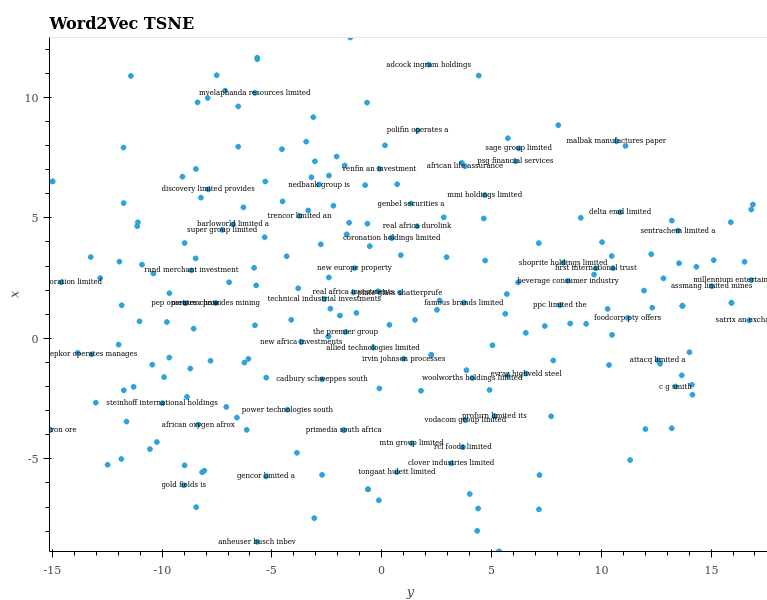
\includegraphics{../experiments/media/Word2Vec TSNE.png}\\

\textbf{Figure 1: Word2vec t-SNE}

When comparing Word2Vec against other techniques we see striking
differences. The first of which is that in techniques like LSI, we see
far stronger clustering of companies with similar names or similar
attributes or description. This is largely attributable to the
underlying methodology in which a Bag-of-Words is reduced to its
dimensionality using some form of Principal Component Analysis (PCA)
with little concern for polysemy. While similar limitations exist in
techniques such as LDA, LDA Hierarchical Bayesian Estimation also lacks
sufficient variation to distinguish strongly between companies.

When assessing Doc2Vec we see the problem of excess noise from article
words whose weighting cannot be reduced in the same way TFIDF does with
Word2Vec, as TFIDF provides more stable and accurate word vectors is
given the size of the corpus.

One reason for the use of Word2Vec over other benchmark techniques is
its ability to provide rich explanation to analysts, its strong use
within the literature and its power in conjunction with many other
techniques such as TFIDF in order to produce documents vectors. Word2Vec
is thus used as the primary technique for the remainder of this paper.

\hypertarget{method}{%
\subsection{Method}\label{method}}

\hypertarget{simplified-method}{%
\subsubsection{Simplified Method}\label{simplified-method}}

Data is sourced from online news articles and grouped into 30-day
news-cycles. A numeric representation for each word in each article is
then computed. Using a description of each company, we take a weighted
sum of each word's numeric representation to compute numeric
representations for each company. The companies are randomly assigned to
1000 portfolios, each consisting of 15 stocks. We calculate the inverse
of the sum of cosine distance between the stocks in the portfolio to
measure the level of similarity between each company. These distances
are then summed for each portfolio to calculate a measure of similarity
between all companies in a portfolio, which we call association. This
metric of association is then used as a measure of portfolio
diversification and compared to the volatility of the portfolio over the
the next 30 days.

\hypertarget{use-of-portfolios-vs-single-stocks}{%
\subsubsection{Use of Portfolios vs Single
Stocks}\label{use-of-portfolios-vs-single-stocks}}

We are using portfolios to analyse risk rather than single stocks for
two reasons. Firstly, risk is reduced in a portfolio by diversifying the
types of assets in the portfolio. The associations made in our model
effectively group stocks by sector. Different sectors have differing
correlations to the market and building portfolios from these grouped
sectors diversifies the portfolio. Secondly, CAPM assumes that Beta
holds only within the context of a well diversified portfolio, but
identifying the diversification of a portfolio remains a complicated
task which no single metric can fully explain and often relies on an
analysts understanding of companies and business and their role in the
underlying economy. Our metric of association aims to quantify these
firm specific attributes to quantify the diversification of a portfolio.

\hypertarget{data-preprocessing}{%
\subsubsection{Data Preprocessing}\label{data-preprocessing}}

\begin{longtable}[]{@{}ccc@{}}
\toprule
& \textbf{Python Computation} &\tabularnewline
\midrule
\endhead
Software & Python 3.6 & Random seed of 42\tabularnewline
Computation & Dask Library & 15 cores, 15 nodes and 30 gigabytes per
node\tabularnewline
\bottomrule
\end{longtable}

Articles were preprocessed by standardizing the text to unicode
characters, before transforming the text into lower-case and removing
all punctuation and numeric characters. The articles were also
preprocessed to remove common stop words in this step. These stopwords
were sourced from the common Scikit-Learn library and included words
like ``the'', ``their'', ``then'' and ``a'', among others. A full list
of packages versions is provided in the appendix.

\hypertarget{model-development}{%
\subsubsection{Model Development}\label{model-development}}

The groups of articles were joined with company descriptions and used to
train a series of Word2Vec models to compute word embeddings on each
trading day. We used Continuous Bag-of-Words (CBOW) Word2Vec model which
was fitted over 30 iterations, using a random seed of 1, a learning rate
of 0.025 and a window of 5.

Given these embeddings, this study makes use of metadata tags of
companies to address the challenge of creating vector representations of
companies. For example, companies like ``AngloGold Ashanti'' are tagged
to concepts such as ``Mining'' in order to ensure robust risk estimation
of thinly cited companies with few mentions in a given news cycle.
Company descriptions were sourced from Bloomberg for use as tags, given
the wide use and reliability of this service. Using word vectors for
each word in a tag computed from our trained models, TFIDF was used to
compute a weighted average of company descriptions. 1000 random evenly
weighted portfolios were drawn, each with 15 stocks and used to
benchmark against against a portfolios forward-looking 30-day
volatility. Backtesting was done on a continuous rolling basis.

One limitation in this study is that these descriptions remain unchanged
over time, while descriptions of companies may have changed during this
time. This may skew the result of this research over certain time
period, where companies have radically changed the nature of their core
operations or where these descriptions are inaccurate.

Using these vector-representations of companies, a cosine distance
metric is used measuring the sum distance between companies within the
portfolio in vector space in order to determine a portfolio risk metric
based on the level of association between them.

Figure 2 presents a t-SNE manifold embedding of the cosine distances
between our different company document vectors. A portfolio of 5
different companies was chosen for illustrative purposes. From this
diagram we can see the edges between nodes representing the distances
between between different points in our portfolio. We expect that
portfolios with longer edges to be more dissimilar and thus to have
greater diversification based on their firm-specific attributes.

\begin{figure}
\centering
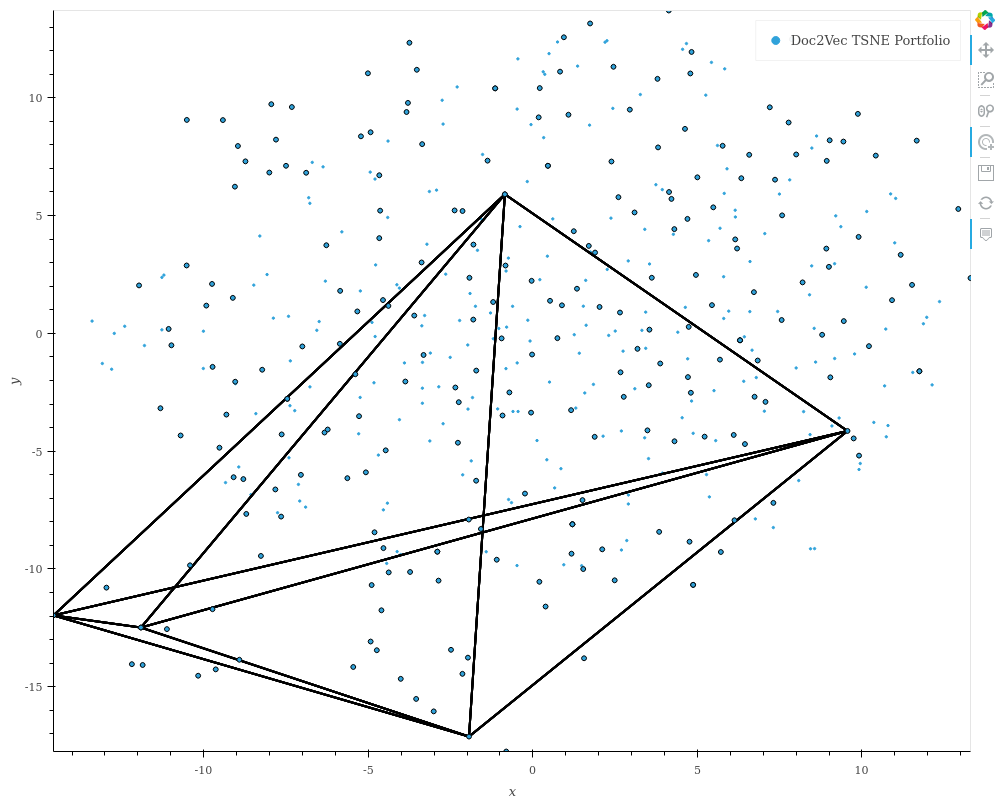
\includegraphics{../experiments/media/Association Computation Diagram.png}
\caption{Association Computation Diagram}
\end{figure}

\textbf{Figure 2: Association Computation Diagram}

Our experimental design makes use of Analysis of Covariance (ANCOVA) in
order to evaluate the relationship between association and portfolio
volatility. ANCOVA will be performed under the assumption of normally
distributed errors. ANCOVA examines the influence of an independent
variable on a dependent variable while removing the effect of the
covariate factor. It assumes a linear relationship between the dependent
variable and the covariate factor. Given the use of continuous testing,
a time series plot of ANCOVA coefficients and p-values will be used to
analyze the relationship between association and volatility.

\[y_{i, j} = \mu + \tau_{i} + \beta (x_{i,j} - \bar{x}) + \epsilon_{i, j} \]

\begin{itemize}
\tightlist
\item
  \(Y_{i, j}\) is the covariate factor
\item
  \(u\) is the grand mean
\item
  \(x\) bar is the global mean\\
\item
  \(x_{i, j}\) is the jth observation of the jth covariate factor\\
\item
  \(t_{i}\) is the variables fitted\\
\item
  \(e_{i, j}\) is the error term.
\end{itemize}

We analyse volume, association and volatility separately and use these
insights to model using ANCOVA. When analysing variance we used ANCOVA
in two different ways. Firstly, we examine variance across portfolios at
a point in time which we denote as ``Date ANCOVA'' and secondly, the
variance within a portfolio over time, ``Portfolio ANCOVA''. Date ANCOVA
performs an ANCOVA by date over all portfolios whilst Portfolio ANCOVA
performs an ANCOVA by Portfolio over all dates in time.

\textbf{Hypothesis}

\[\text{H}_{0}: \beta_{1} = 0 \]\\
\[\text{H}_{1}: \beta_{0} = 0 \]

Where \(\beta_{1}\) is a measure of association of a given portfolio at
a point in time.

\hypertarget{results-and-discussion}{%
\section{Results and discussion}\label{results-and-discussion}}

\hypertarget{volume-and-association}{%
\subsection{Volume and association}\label{volume-and-association}}

In analysing news volume over time it is clear that the volume of news
articles scraped before 2009 is extremely low, increasing slowly up
until 2014 with a rapid spike into 2018. Figure 3 details word vector
associations over time. These seem to appear completely constant, before
beginning to differ from 2008 onwards. This is due to the number of news
articles used increasing dramatically during this period, which remains
a limitation of this study. Figure 4 details the volume plot and is
related to the association plot in that as news article volume increases
so does the stability and accuracy of word vectors used to compute
association.

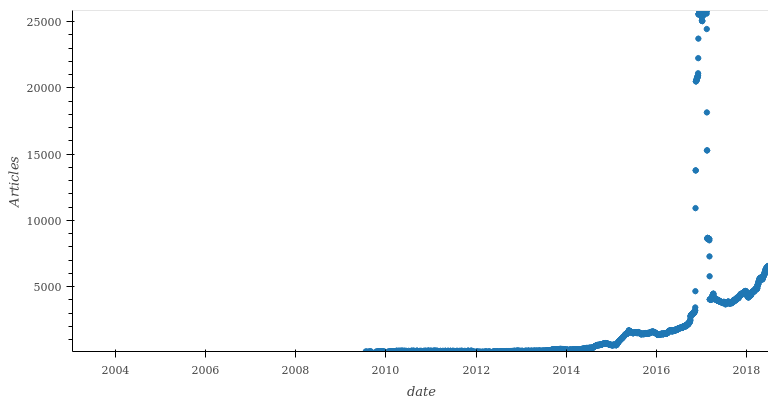
\includegraphics{../experiments/media/News Volume.png}

\textbf{Figure 3: News Volume}

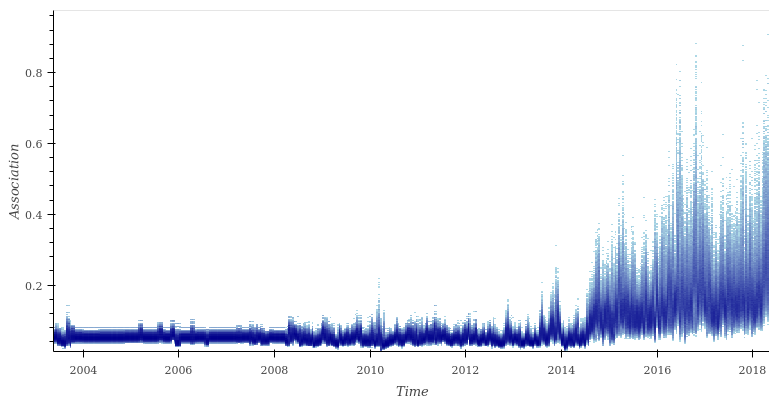
\includegraphics{../experiments/media/Association Over Time.png}\\

\textbf{Figure 4: Association}

Volatility details the standard deviation of portfolios over time.
Figure 5 details the 300-day volatility of returns across 1000 random
evenly weighted portfolios between 16 May 2003 and 17 May 2018. When
assessing volatility over time the influence of macroeconomic events
such as the financial crisis in 2008 and the South African ``Zuma-gate
scandal'' of 2016 are attributed to the spikes in portfolio volatility.

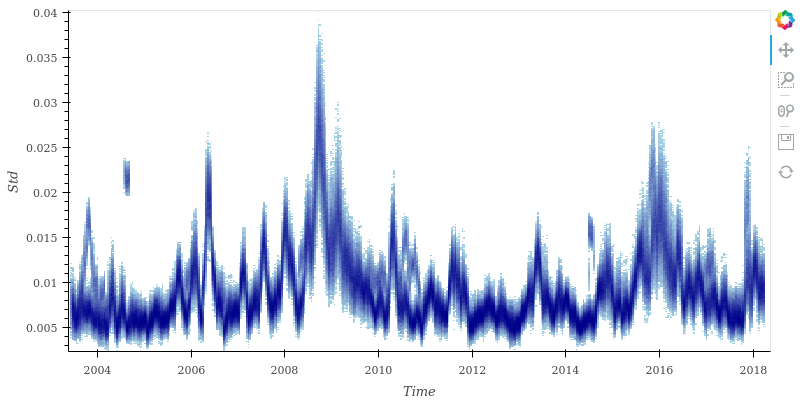
\includegraphics{../experiments/media/Volatility Over Time time.png}\\

\textbf{Figure 5: Volatility}

\hypertarget{date-ancova}{%
\subsection{Date ANCOVA}\label{date-ancova}}

In running a test to determine whether a relationship between
association and volatility exists at a singular point in time, the model
is found to be insignificant. However, it is difficult to conclude from
this result alone that the effect of association on portfolio
diversification and volatility is entirely insignificant.

Figure 6 details how our coefficients and constant in the model change
across portfolios at specific points in time, referred to as ``Date
ANCOVA''. Data is observed between 2011 and 2018 due to the sparsity of
articles captured before these dates as outlined in Figure 2. The
coefficients depict an erratic motion with no real pattern or
seasonality present. This may signify either the presence of some latent
source of variation not captured by the model or the effects of random
sampling. The coefficients are zero at many points in time violating the
hypothesis for the model as coefficients equalling zero will have no
effect on the model. When assessing the significance of the model across
portfolios at points in time, in Figure 7, we find that our coefficient
p-values are extremely large on average and that the majority of
portfolios are not significant at the 5\% level. This means that there
is no evidence to reject the null hypothesis and we make the assumption
that \(\beta_{1}=0\), implying coefficients are not useful in the model.

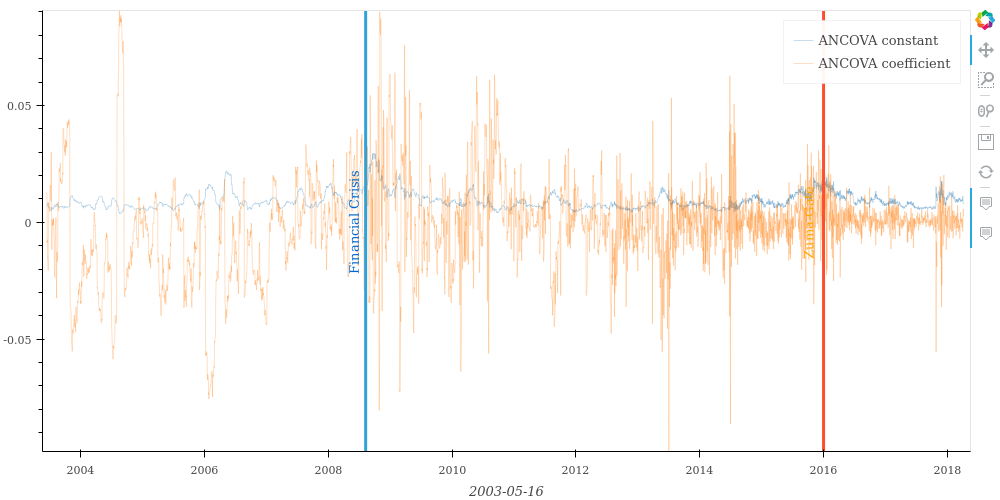
\includegraphics{../experiments/media/Coefficients with constant over time.png}\\

\textbf{Figure 6: Coefficients Across Portfolios at Points in Time}

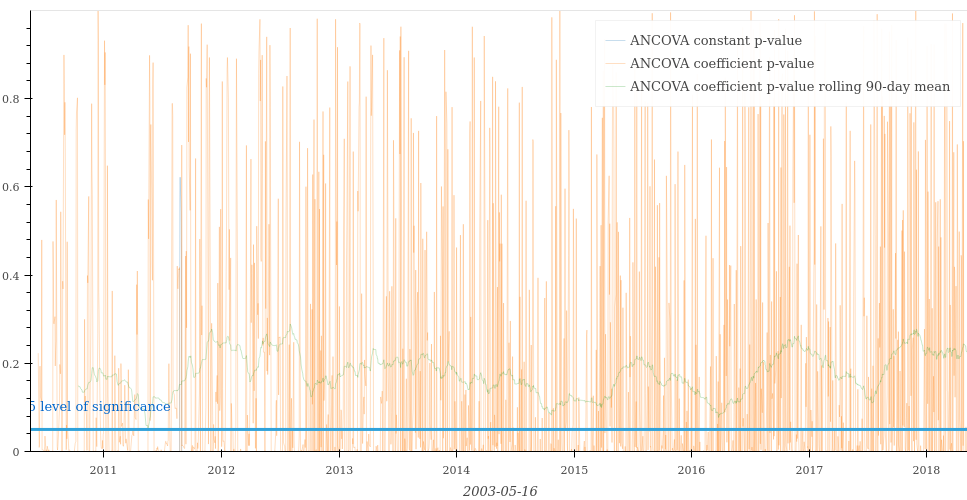
\includegraphics{../experiments/media/P-Values with constant over time.png}\\

\textbf{Figure 7: Coefficent P-values Across Portfolios at Points in
Time}

In order to understand why these results may be insignificant we analyse
the distribution of our portfolios at some random point in time. Figure
8 and Figure 9 details results from 21/03/2015, a random date in our
sample. The Figure 8 and Figure 9 show no trend and exhibit a completely
random and uninterpretable array of points. The results show an
extremely low R-squared value of 0.004, which explains how much
variation in volatility is explained by our association metric, and even
though R-squared is not an exhaustive measure of model validity, it is
clear to see that volatility is explained extremely poorly by
association. The t-stat for the coefficient, used to infer if there is
significant variation between the means of two groups is low at 2.118
which is why the p-value is so high in the model even though the
constant is significant and, inevitably, why the results are so
insignificant.

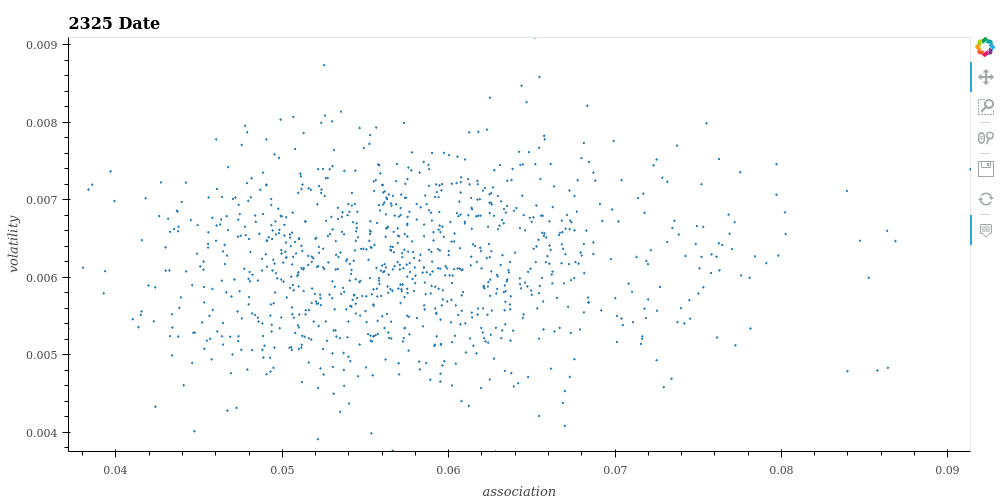
\includegraphics{../experiments/media/Scatter Plot of Portfolios on 2014-03-21.png}\\

\textbf{Figure 8: Scatter Plot of Portfolio Association and Volatility
as at 2014/03/21}

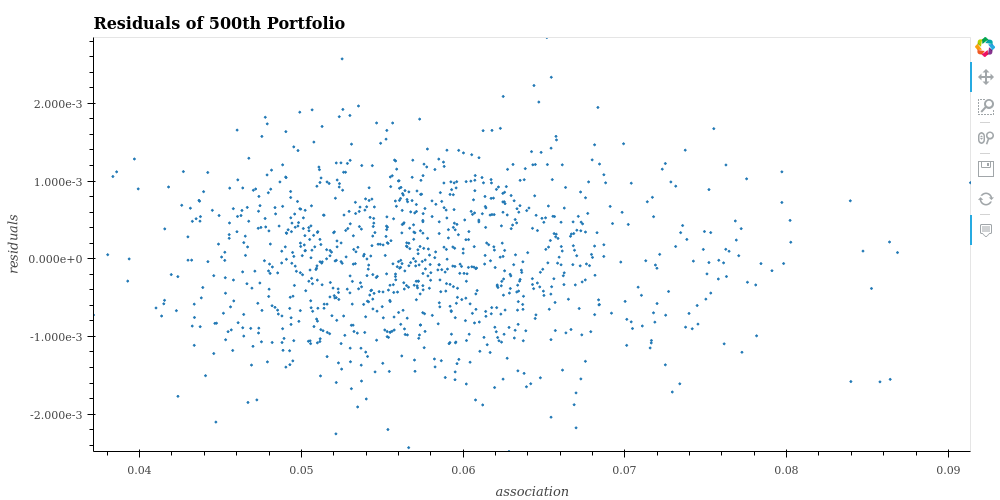
\includegraphics{../experiments/media/Scatter Plot of Residuals of Portfolios on 2014-03-21.png}\\

\textbf{Figure 9: Scatter Plot of Portfolio Association and Residuals as
at 2014/03/21}

\begin{longtable}[]{@{}lllllll@{}}
\toprule
& & \textbf{Table 2} & & & &\tabularnewline
\midrule
\endhead
Dep. Variable & y & & & R-squared & 0.004 &\tabularnewline
Method: & Least Squares & & & Adj. R-squared & 0.003 &\tabularnewline
No.~Observations: & 1000 & & & F-statistic & 4.486 &\tabularnewline
DF Residuals: & 998 & & & Prob(F-statistic) & 0.0344 &\tabularnewline
Df Model: & 1 & & & Log-likelihood & 5684.4 &\tabularnewline
Covariance type & non-robust & & & AIC: & -1.136e+04 &\tabularnewline
& & & & BIC: & -1.136e+04 &\tabularnewline
& & & & & &\tabularnewline
& Coef & std err & t & \(p>|t|\) & {[}0.025 0.975{]} &\tabularnewline
constant & 0.0058 & 0.000 & 32.799 & 0.000 & 0.005 &
0.006\tabularnewline
X1 & 0.0064 & 0.003 & 2.118 & 0.034 & 0.000 & 0.012\tabularnewline
\bottomrule
\end{longtable}

Due to the preceding results we are inclined to believe that portfolios
comprise of many sources of volatility which arise in the inclusion of a
particular share with high volatility, market microstructure or a
variety of other effects. In order to further explore the relationship
between association and volatility we propose the analysis of portfolios
over time, a method by which to control for these factors affecting the
volatility of a specific portfolio.

We propose looking at ANCOVA across time in particular portfolios,
``Portfolio ANCOVA'', which will isolate our volatility factor, in order
to find a trend in the data when accessing volatility and residuals.

\hypertarget{portfolio-ancova}{%
\subsection{Portfolio ANCOVA}\label{portfolio-ancova}}

The Portfolio ANCOVA coefficients, observed in Figure 10, are reasonably
uniformly distributed, are all positive and lie in a reasonable range
which suggests that the model is significant. The same can be said for
the ANCOVA constant x-values which exhibit similar traits, in Figure 11.
The coefficient p-value plot (figure something 12) shows that for the
majority of time periods the portfolios are significant at the 1\% level
with fewer portfolios significant at the the 5\% level. This is
sufficient evidence to reject the null hypothesis that conclude that
\(\beta_{1}\) is not equal to 0 which means that the coefficients will
add to variation in volatility. This provides evidence that there is
covariance in coefficients but does not explain the magnitude of the
coefficients.

\includegraphics{../experiments/media/Coefficeint Value with contant accross portfolio.png}\\

\textbf{Figure 10: Coefficients Across Time Within Portfolios}

\includegraphics{../experiments/media/Coefficeint value with contant accross portfolio.png}

\textbf{Figure 11: Constants Across Time Within Portfolios}

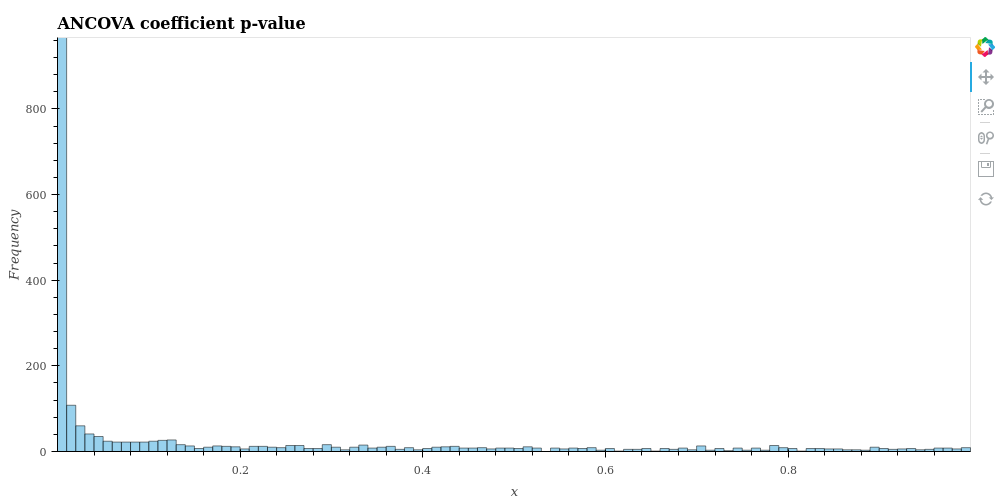
\includegraphics{../experiments/media/Coefficeint P-value with contant accross portfolio.png}\\

\textbf{Figure 12: Coefficient P-values Across Time Within Portfolios}

In order to understand why these results may be significant we analyse
the distribution of a portfolio over time, this being the 500th
portfolio. We assess association and how it affects volatility and
residuals. In these plots there is a definite trend. In the Figure 13
there is a clear clustering of days where both association and
volatility are low and the density of days decreases as both volatility
and association increase. The residuals plot, shown in Figure 14, is
similar with a large cluster at an association below 0.1 and thinning
out as association increases. This suggests a positive relationship
between association and volatility. With an R-squared value of 0.068,
this is not much better than the previous method but it is improved
which shows greater explanation of volatility by association, on
average. The telling statistic is the t-stat, which in this method is
sufficiently large enough for the coefficient and the constant, making
p-values significantly small.

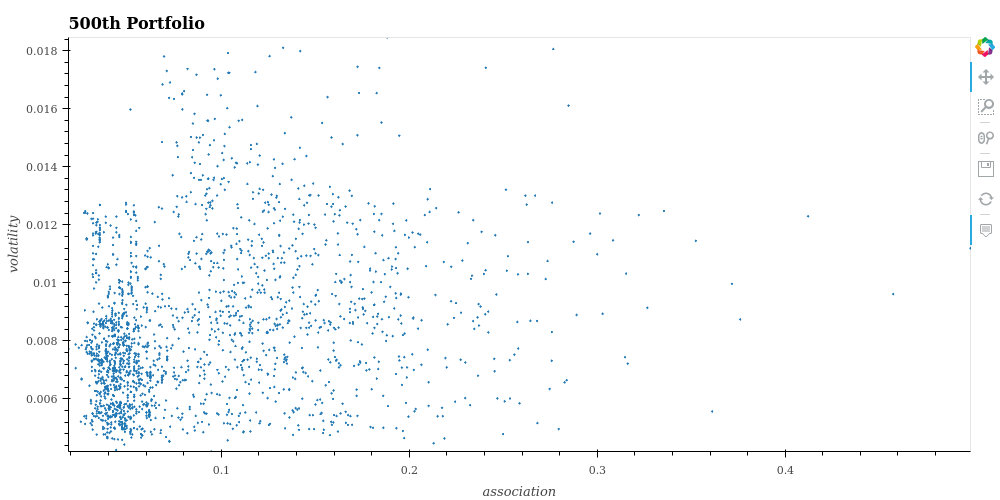
\includegraphics{../experiments/media/Scatter Plot of 500th Portofolio.png}\\

\textbf{Figure 13: Scatter Plot of Association and Volatility of the
500th Portfolio}

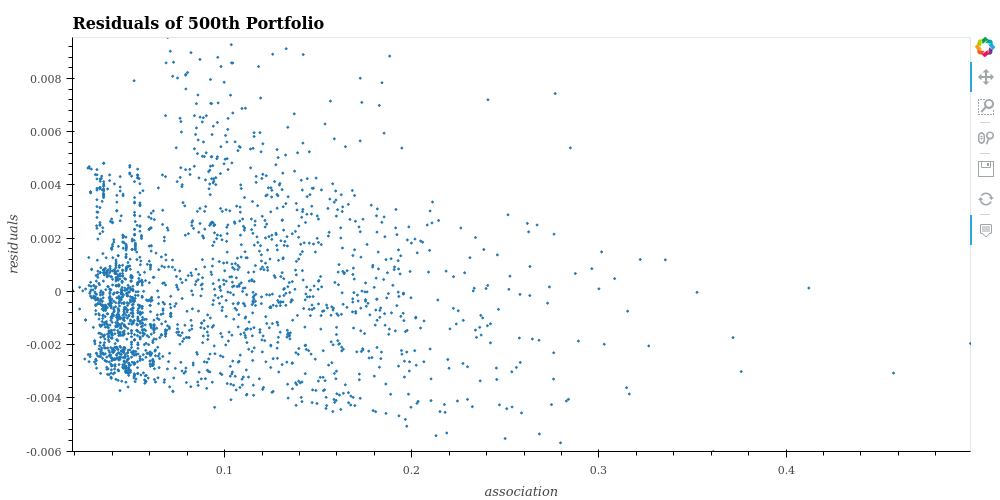
\includegraphics{../experiments/media/Scatter Plot of Residuals of 500th Portofolio.png}\\

\textbf{Figure 14: Scatter Plot of Association and Residuals of the
500th Portfolio}

\begin{longtable}[]{@{}lllllll@{}}
\toprule
& & table 3 & & & &\tabularnewline
\midrule
\endhead
Dep. Variable & y & & & R-squared & 0.068 &\tabularnewline
Method: & Least Squares & & & Adj. R-squared & 0.068 &\tabularnewline
No.~Observations: & 2058 & & & F-statistic & 150.8 &\tabularnewline
DF Residuals: & 2056 & & & Prob(F-statistic) & 1.70e-33 &\tabularnewline
Df Model: & 1 & & & Log-likelihood & 9334.1 &\tabularnewline
Covariance type & non-robust & & & AIC: & -1.866e+04 &\tabularnewline
& & & & BIC: & -1.865e+04 &\tabularnewline
& & & & & &\tabularnewline
& Coef & std err & t & \(p>|t|\) & {[}0.025 & 0.975{]}\tabularnewline
constant & 0.0075 & 0.000 & 72.687 & 0.000 & 0.007 &
0.008\tabularnewline
X1 & 0.0114 & 0.001 & 12.279 & 0.000 & 0.010 & 0.013\tabularnewline
\bottomrule
\end{longtable}

\hypertarget{incorporation-of-blocking}{%
\subsection{Incorporation of blocking}\label{incorporation-of-blocking}}

Through an analysis of Date ANCOVA and Portfolio ANCOVA, this paper has
identified that portfolios contain many sources of variation. We have
concluded the two main sources of variance to be excess systematic
volatility on a given day and excess volatility of a particular share in
a portfolio. We therefore propose a third method in which to control for
these sources of variance using blocking.

Using data on shares in in our portfolios we propose a model to test for
these sources of variation jointly, shown in the equation below:\\
\[ y = \beta_{0} + \beta_{1} \text{Association} +  \sum_{i=1}^{t} \beta_{i} x_{i}+ \sum_{j=1}^{c} \beta_{j} x_{j} + \epsilon_{i, j}  \]

Where \(t\) represents a trading day in our dataset and \(c\) represents
the companies in a given portfolio.

Given the number of data points, a stratified sample of our data was
taken in order to fit this model. The results are shown in the table
below:

\begin{longtable}[]{@{}lllllll@{}}
\toprule
& & table 4 & & & &\tabularnewline
\midrule
\endhead
Dep. Variable & y & & & R-squared & 0.794 &\tabularnewline
Method: & Least Squares & & & Adj. R-squared & 0.790 &\tabularnewline
No.~Observations: & 123450 & & & F-statistic & 182.6 &\tabularnewline
DF Residuals: & 120899 & & & Prob(F-statistic) & 0.000 &\tabularnewline
Df Model: & 2550 & & & Log-likelihood & 6.2152e+05 &\tabularnewline
Covariance type & non-robust & & & AIC: & -1.238e+64 &\tabularnewline
Date & Mon, 17 Sep 2018 & & & BIC: & -1.213e+06 &\tabularnewline
Time & 23:56:13 & & & & &\tabularnewline
& Coef & std err & t & \$p\textgreater{} & t & \$\tabularnewline
Association & 0.007 & 0.000 & 3.529 & 0.000 & 0.000 &
0.001\tabularnewline
\ldots{} & & & & & &\tabularnewline
Constant & 0.0024 & 4.84e-06 & 500.510 & 0.000 & 0.002 &
0.002\tabularnewline
& & & & & &\tabularnewline
Omnibus: & 25356.151 & Skew: & 0.933 & Dubin-Watson & 1.999
&\tabularnewline
Prob(Omnibus): & 0.000 & Kurtosis: & 7.402 & Jarque-Bera (JB): &
117583.806 &\tabularnewline
Prob(JB): & 0.000 & Cond. No. & 1.72e+17 & & &\tabularnewline
\bottomrule
\end{longtable}

From the 120899 observations, we can observe a constant value of 0.0024
and an association coefficient of 0.0007, both significant at the 0.1\%
level, with t-scores of 500.510 and 3.529 respectively. This model
demonstrates a \(R^2\) value of 0.794 and joint-significance of 182.6
which is significant at the 0.1\% level using Fisher's F-statistic. If
we then analyze the residuals of this model, shown in Figure 15, we
observe their distribution as both symmetric and distributed around 0,
with little correlation to association, shown in Figure 15. These
properties are crucial to Gauss-Markov Assumptions of Ordinary Least
Squares Linear Regression and the use of these estimates as an unbiased
linear estimator of portfolio variance. The p-values of our date
coefficient under the null hypothesis \(\beta_{t} = 0\) are both
significant and insignificant at points in time, suggesting the effect
of exogenous shocks to our model, shown in Figure 17. Despite these
findings, we see using blocking to control for a share's excess
volatility, demonstrating significant p-values at the 0.001\% level
using the student t-distribution, providing strong argument for their
use in this blocking design, shown in Figure 18.

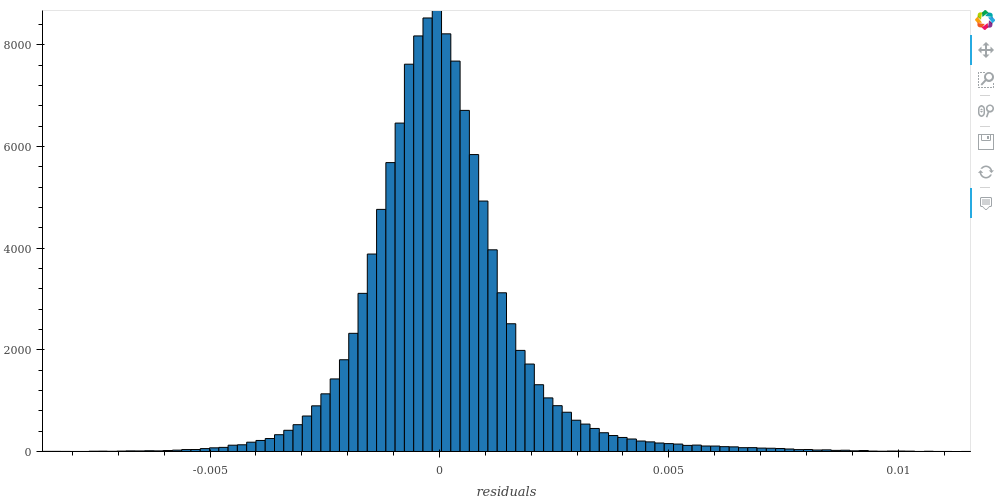
\includegraphics{../experiments/media/Histogram of Residuals of Blocking Ancova.png}\\

\textbf{Figure 15: Histogram of Residuals for the Blocking ANCOVA}

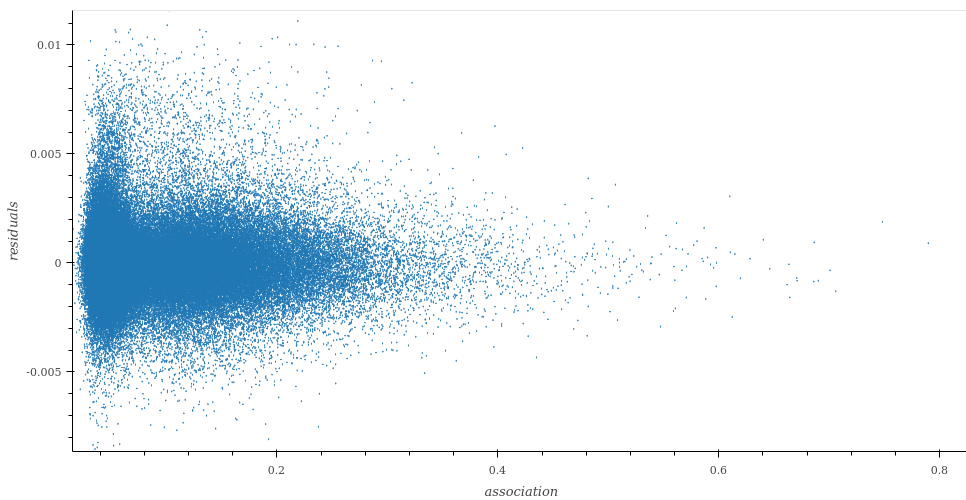
\includegraphics{../experiments/media/Scatter Plot of Residuals of Blocking Ancova.png}\\

\textbf{Figure 16: Scatter Plot of Association and Residuals Blocking
ANCOVA }

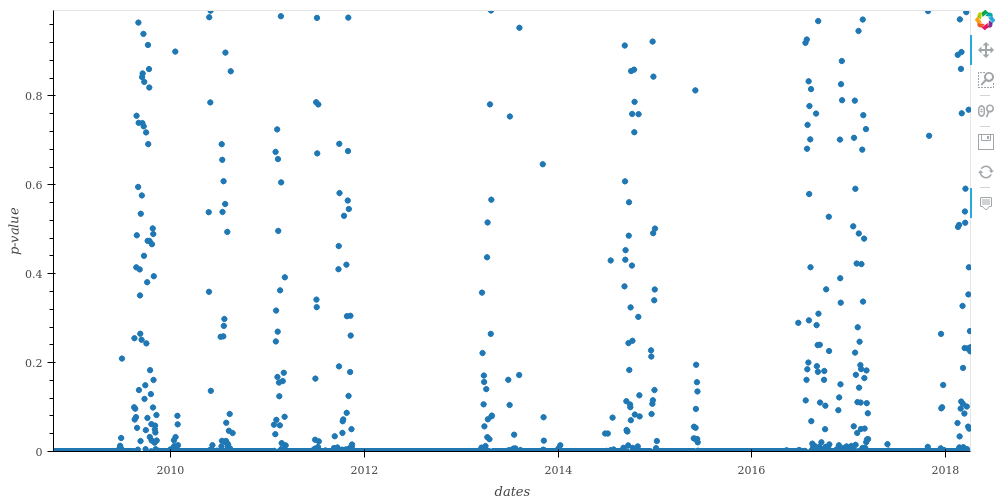
\includegraphics{../experiments/media/Scatter Plot of P-values for dates of Blocking Ancova.png}\\

\textbf{Figure 17: Scatter Plot of P-values for Dates of Blocking ANCOV}

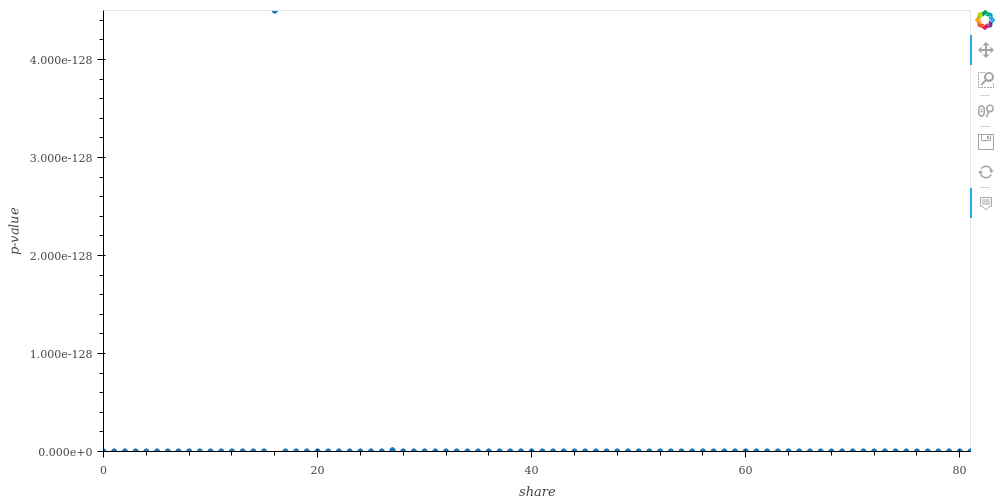
\includegraphics{../experiments/media/Scatter Plot of P-values for shares in a portfolio of Blocking Ancova.png}\\

\textbf{Figure 18: Scatter Plot of P-values for Portfolios of Blocking
ANCOVANCOVA}

\hypertarget{conclusions}{%
\section{Conclusions}\label{conclusions}}

CAPM states systematic risk to be the sole risk determinant of returns,
given efficient markets, where non-systematic risk is perfectly
diversifiable. In reality however, markets are shown not to perfectly
efficient. Given this lack of efficiency it holds that investments are
subject to non-systematic risk, such as the size and value effect. This
paper contributes to the existing literature, offering association risk
as a portfolio specific anomaly identifying the level of diversification
within a portfolio and hence its volatility in the market.

The relationship between company association of shares within a
portfolio on the Johannesburg Stock Exchange and portfolio volatility is
confirmed by the results of this study. Firstly, Date ANCOVA produces a
highly insignificant model which could not isolate association as a
determinant of volatility without sufficient control of additional
sources of volatility. However, using Portfolio ANCOVA the noise is
eradicated over time and association is isolated producing significant
results. Whilst we are confident that covariance is not equal to zero,
the extent to how much the coefficients vary make it inappropriate for
use in predictive applications. Finally, using our blocking experimental
design, we find a strong argument for the relationship between
association and portfolio variance, when controlling for excessive
systematic variance at points in time and contributions of variance by
outlying high volatility shares.

An opportunity for future research exists in which association risk
could be used in predictive modeling and portfolio optimisation.

    \hypertarget{appendix}{%
\section{Appendix}\label{appendix}}

\hypertarget{tf-idf}{%
\subsection{TF-IDF}\label{tf-idf}}

TF-IDF is an information retrieval technique that weighs a term's
frequency (TF) and its inverse document frequency (IDF). Each term has
its respective TF and IDF score and the product of the scores is the
TF-IDF weight of that term. The higher the score the rarer the term and
vice versa. This score is used to assign the importance of the term
throughout the the corpus. For a term t in a document d, the weight Wt,d
of term t in document d is given by:

\(W_{t,d} = TF_{t,d} log(N/DF_{t})\)

Where:\\
- \(TF_{t,d}\) is the number of occurrences of \(t\) in document
\(d\).\\
- \(DF_{t}\) is the number of documents containing the term \(t\).\\
- \(N\) is the total number of documents in the corpus.

\hypertarget{word2vec}{%
\subsection{Word2Vec}\label{word2vec}}

The easiest way to think about word2vec is that it figures out how to
place words on a ``chart'' in such a way that their location is
determined by their meaning, called a vector-space. This means that
words with similar meanings will be clustered together. I.e.: Words with
semantic relationships will be closer together than words without such
relationships. Word2vec is a three-layer neural network with one input,
one hidden and an output layer. Word2vev can utilize Continuous bag of
words (CBOW) or continuous skip-gram architecture. The idea of CBOW
(continuous bag-of-words) architecture, the Word2vec algorithm we are
using, is to learn word representations that can predict a word given
its surrounding words. The input layer corresponds to signals for
surrounding words and output layer correspond to signals for predicted
target word. Suppose, you have an input sentence: ``The cat sat on the
mat''. The aim is to learn representation for words ``the'', `'cat'',
``sat'' etc. To this end, the neural network tries to learn features
(weights W and W′) which look at words in a window, say ``The cat sat''
and try to predict the next word, ``on''. Hence, with input as the
``the'', `'cat'', `'sat'', the training process adjusts the weight of
the network, so that the probability of output ``on'' is maximized, as
compared to other words in the vocabulary. As the training procedure
repeats this process over large number of sentences or phrases, the
weights ``stabilize''. These weights are then used as the vectorized
representations of words.

\hypertarget{word2vec-1}{%
\subsection{Word2vec}\label{word2vec-1}}

\begin{figure}
\centering
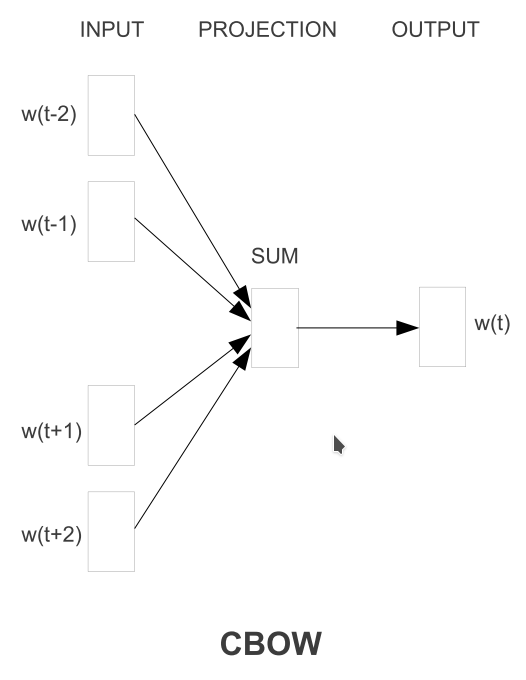
\includegraphics{../experiments/media/Word2Vec CBOW.png}
\caption{Word2vec CBOW}
\end{figure}

{[}@Mikolov2013a{]}

The CBOW architecture predicts the current word based on context of a
given word.

\begin{figure}
\centering
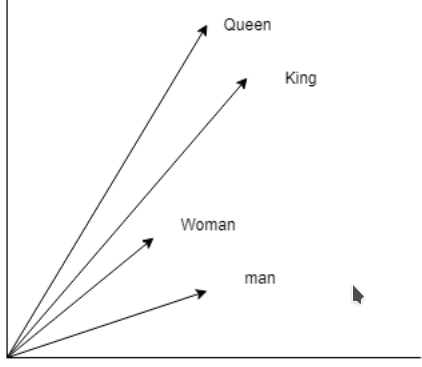
\includegraphics{../experiments/media/Word2vec simplified.png}
\caption{Simplified Word2vec}
\end{figure}

This diagram outlines the vector relationship maintained through the use
of word embeddings.\\
king - man + woman = queen

\hypertarget{negative-sampling}{%
\subsection{Negative Sampling}\label{negative-sampling}}

Negative-sampling is a method by which samples are drawn outside a given
distribution. In the context of Word2Vec and Doc2Vec embedding
techniques, this involves sampling incorrect contexts for a given word
or incorrect document tags for a given document to be used as false
labels when training the embedding model.

\hypertarget{doc2vec}{%
\subsection{Doc2vec}\label{doc2vec}}

Doc2vec is an adaption of Word2vec but instead of generating
relationships between words it generates relationships between
paragraphs, sentences and documents. Again, there is a three-layer
neural network with an input, a hidden and an output layer. The
difference is that in the input layer there is now a signal for the
document as well as the signals for surrounding words which is what
makes the distinction between documents. The output layer, again,
corresponds to signals predicting target words.

\hypertarget{lda}{%
\subsection{LDA}\label{lda}}

Latent Dirichlet Allocation (LDA) is a generative statistical model that
allows sets of observations to be explained by unobserved groups that
explain why some parts of the data are similar. For example, an LDA
model might have topics classified as finance-related and
mining-related. Topics have probabilities of generating various words
such as ore, gold, strikes which can be classified and interpreted by
the viewer as mining-related. Likewise, the finance-related topic has
probabilities of generating words commonly associated with finance.
Words without relevance will have roughly equal probabilities. A lexical
word may occur in several topics with a different probability but with a
different typical set of neighbouring words in each topic. Each document
is assumed to be characterized by a set of topics which makes the
individual words exchangeable.

\hypertarget{lsi}{%
\subsection{LSI}\label{lsi}}

Latent Semantic Indexing (LSI)is a technique of analysing relationships
between a set of documents and the terms they contain by producing a set
of concepts related to the documents and terms. LSI assumes that words
that are close in meaning will occur in similar pieces of text. A matrix
containing word counts per paragraph is constructed from a large piece
of text and a mathematical technique called Singular Value Decomposition
is used to reduce the number of rows while preserving the similarity
structure among columns. Words are then compared by taking the cosine of
the angle between the two vectors formed by any two rows. Values close
to 1 represent very similar words while values close to 0 represent very
dissimilar words.

\hypertarget{companies-in-the-analysis}{%
\section{Companies in the analysis}\label{companies-in-the-analysis}}

`ACL', `AEG', `AEL', `AFE', `AFX', `AGL', `AMS', `ANG', `APN', `ARI',
`ASR', `AVI', `AXL', `BAT', `BAW', `BGA', `BIL', `BVT', `CAT', `CLS',
`CML', `CPI', `DRD', `DST', `DSY', `DTA', `DTC', `EOH', `EXX', `FBR',
`FSR', `GFI', `GND', `HAR', `HCI', `IMP', `INL', `INP', `IPL', `KAP',
`LBH', `LON', `MMI', `MRF', `MRP', `MSM', `MTN', `MUR', `NED', `NHM',
`NPK', `NPN', `NTC', `OCE', `OML', `OMN', `PBG', `PIK', `PPC', `PSG',
`RCL', `REM', `RLO', `RMH', `SAP', `SBK', `SHP', `SLM', `SNH', `SNT',
`SOL', `SPG', `SUI', `TBS', `TFG', `TKG', `TON', `TRE', `TRU', `TSH',
`WBO' and `WHL'.

\hypertarget{smacof}{%
\section{SMACOF}\label{smacof}}

\[\sigma(X) = \sum_{i<j<n} w_{i,j} (d_{i,j}(X)-\delta_{i,j})^2 =\sum_{i<j}(w_{i,j} \delta_{i,j}^2) + \sum_{i<}w_{i,j} d_{i,j}^2 (X) - 2 \sum_{i<j}w_{i,j} \delta_{i,j} d_{i,j}(X)\]

SMACOF uses an algorithm called majorizing to minimise stress functions.
Strictly speaking majorization is not an algorithm but rather an
approach to constructing optimization algorithms. The principle of
majorization is to construct a surrogate function which
majorizes/minimizes a particular function. In some optimizations
problems, the objective-function is just too complicated to evaluate
directly at every iteration. Surrogate functions are constructed to
mimic most of the properties of the true objective-function, but that is
much simpler analytically and/or computationally.

TSNE

t-ditribution stochastic neighbour embedding (t-SNE)

t-SNE is a tool to visualize high-dimensional data. It converts
similarities between data points to joint probabilities and tries to
minimize the Kullback-Leibler divergence between the joint probabilities
of the low-dimensional embedding and the high-dimensional data. t-SNE
has a cost function that is not convex, i.e.~with different
initializations we can get different results.

\hypertarget{graphs}{%
\section{Graphs}\label{graphs}}

\hypertarget{exploratory-data-analysis-plots}{%
\subsection{Exploratory Data Analysis
Plots}\label{exploratory-data-analysis-plots}}

\begin{figure}
\centering
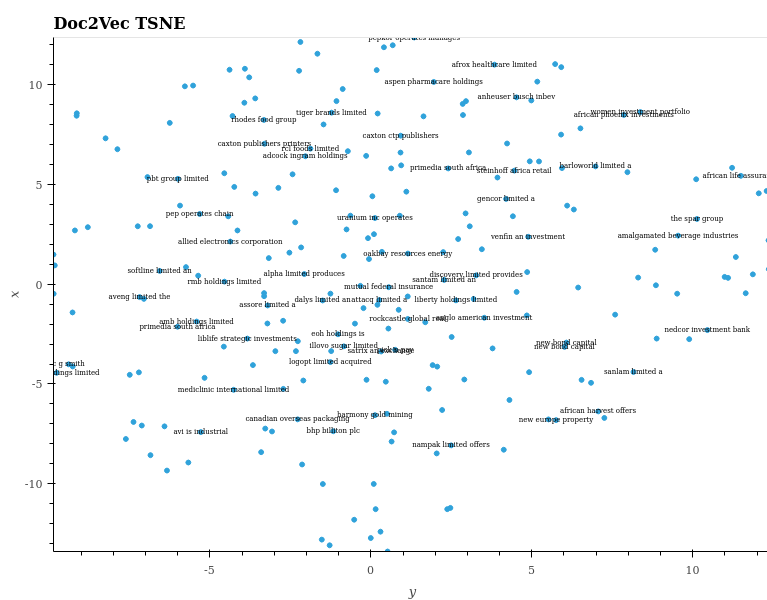
\includegraphics{../experiments/media/Doc2Vec TSNE.png}
\caption{Doc2vec t-SNE}
\end{figure}

\begin{figure}
\centering
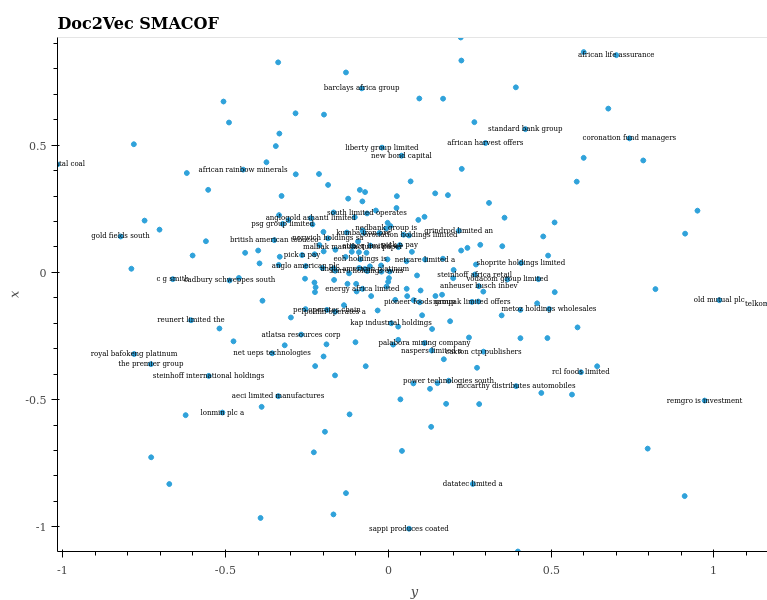
\includegraphics{../experiments/media/Doc2Vec SMACOF.png}
\caption{Doc2vec SMACOF}
\end{figure}

\begin{figure}
\centering
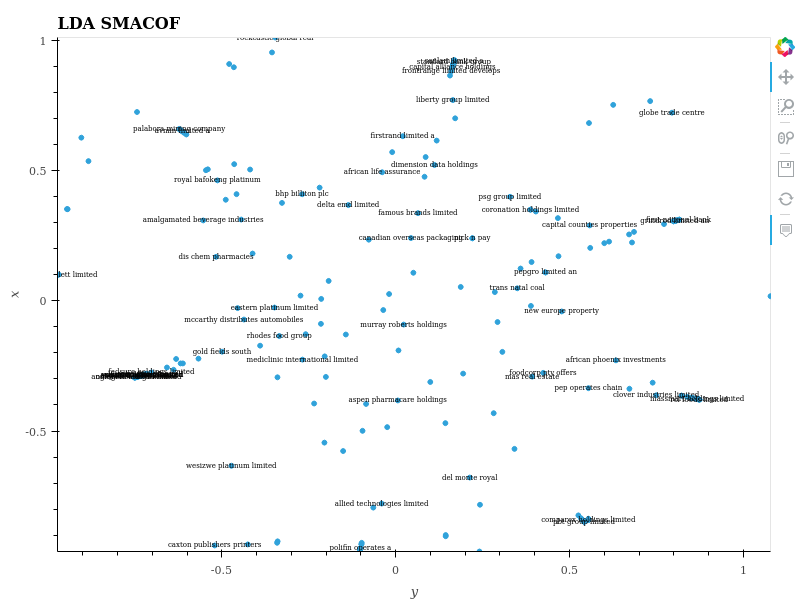
\includegraphics{../experiments/media/LDA SMACOF.png}
\caption{LDA SMACOF}
\end{figure}

\begin{figure}
\centering
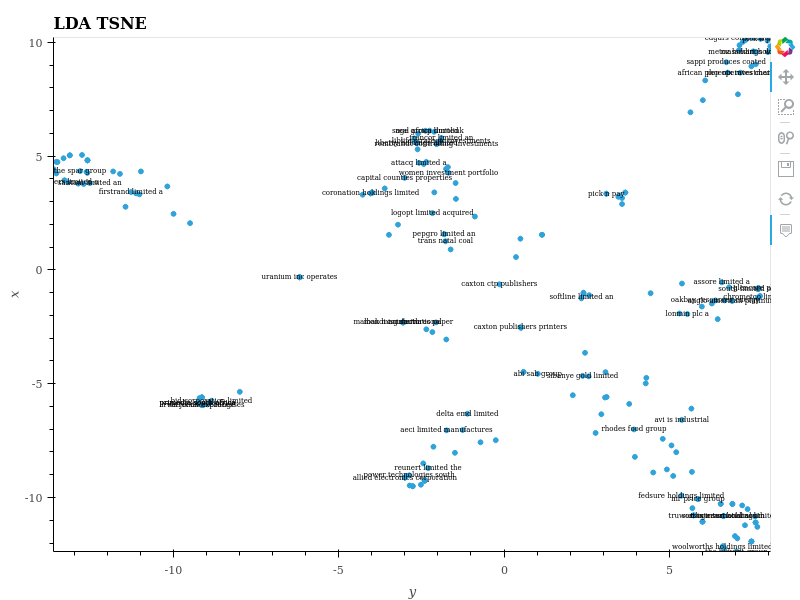
\includegraphics{../experiments/media/LDA TSNE.png}
\caption{LDA t-SNE}
\end{figure}

\begin{figure}
\centering
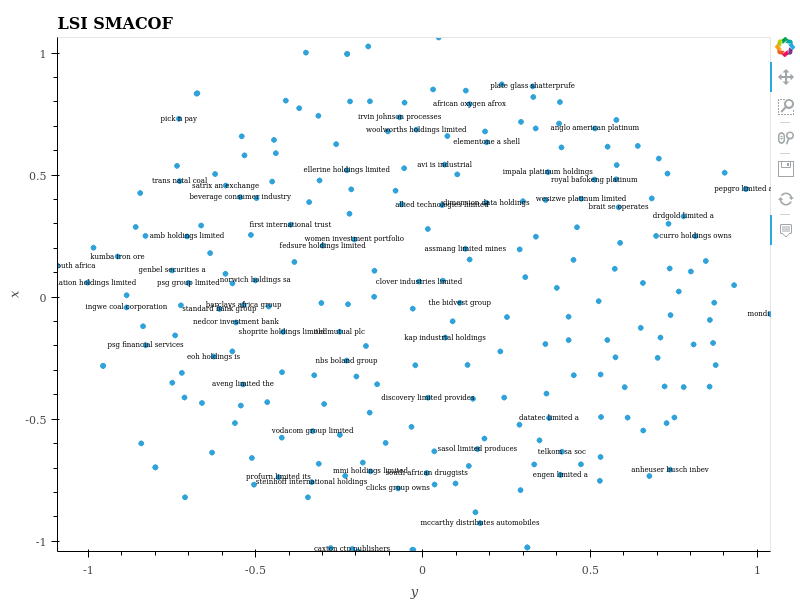
\includegraphics{../experiments/media/LSI SMACOF.png}
\caption{LSI SMACOF}
\end{figure}

\begin{figure}
\centering
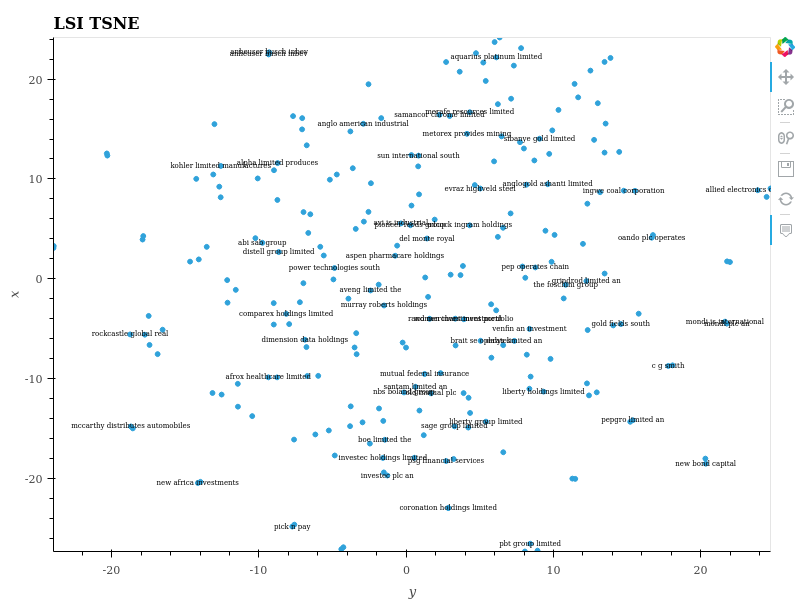
\includegraphics{../experiments/media/LSI TSNE.png}
\caption{LSI t-SNE}
\end{figure}

\begin{figure}
\centering
\includegraphics{../experiments/media/Constant P-value with contant accross portfolio.png}
\caption{Constant P-values Across Time Within Portfolios}
\end{figure}

    \hypertarget{references}{%
\section{References}\label{references}}


    % Add a bibliography block to the postdoc
    
    
    
    \end{document}
